\chapter{Contribution}
\label{sec:contribution}

In the current chapter, contribution during Master Thesis is presented.
As result, a GNN can be presented which is called \textit{GAT-Denoiser}.
Its main components and the overall architectur is introduced.

The focus during practical part was on classical computed tomography in 2D but
can be generalized to cryo-EM and 3D.

\paragraph{Goal}
As introduced in chapter~\ref{sec:imaging}, molecular imaging methods computed tomography and cryo-EM are the problems
to approach. Further, the high-noise regime is the domain of interest, to be more precise SNR between $[-20, 0]$.

For a given set of observations (many sinograms or micrographs), a GNN will be trained, such that
it enables denoising of observations which are expected to have better reconstruction results.
The trained model allows to denoise not seen observations, which are from the same family of observations.


\begin{tcolorbox}[colback=red!5!white,colframe=red!75!black]
  To start solving the problem, an algorithm was designed to work with computed tomography, additionally
  projection angles are assumed to be known and $\theta$ was defined as equally spaced 
  in the inverval $[0, 2 \pi]$. \\
\end{tcolorbox}

\paragraph{Input graph:}
To recap from section~\ref{sec:graphConstruction}, our graph from molecular-imaging observation
will have single observations as nodes (one horizontal line of the sinogram). 
As $\theta$ is fixed, angle corresponding to each single observation are known. 
Based on these angles, neighbouring nodes can be connected.

\begin{tcolorbox}[colback=red!5!white,colframe=red!75!black]
  For GAT-Denoiser, this means that graph topology is fixed. 
  A K-NN graph can be built from points, equally spaced on the unit-circle,
  as signal of observations is assumed to process the low-dimensional manifold.
\end{tcolorbox}


\section{Concept}


In the following section, the concept of GAT-Denoiser is introduced. 
GAT-Denoiser is a GNN and has two main components, namely convolution layers and GAT layers.
The main idea of GAT-Denoiser is to enable denoising of observations:
\begin{equation}
  \text{GAT-Denoiser} (\cdot) : L^2(\tilde{\Omega}) \to  L^2(\tilde{\Omega}) , y \mapsto \text{GAT-Denoiser} (y) 
\end{equation}

% The GAT is expected to denoise observation signal with its neighbours by averaging. 
% Further, convolution is added to denoise single observations.

\begin{figure}[H]
  \centering
  \label{fig:overall-concept}
  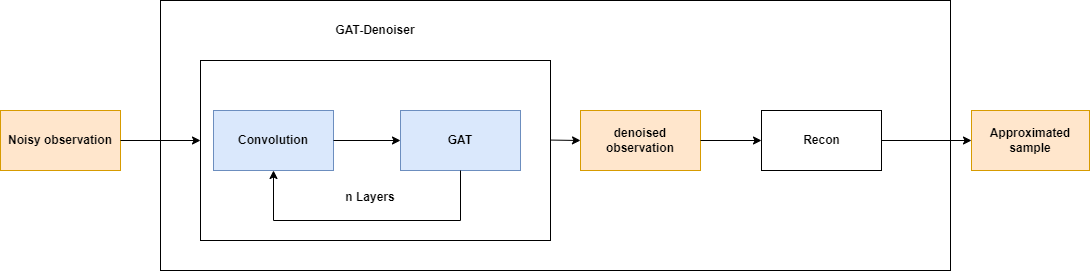
\includegraphics[width=\textwidth]{Overall_GAT-Denoiser_Pipeline.drawio.png}
  \caption{GAT-Denoiser concept}
\end{figure}

\textbf{TODO: Add REcon box}

In figure~\ref{fig:overall-concept}, the overall GAT-Denoiser concept is illustrated.
The input of the GAT-Denoiser network is a noisy observation, the output will be a denoised version.

GAT will be responsible to average over observation neighbours, but single observations will
not be averaged by the GAT. 
Therefore, convolution is added and is responsible to denoise single observations
before averaging over neighbourhood with GAT. So for every GAT layer, there is a preceding convolution. 
In the case of computed tomography, this will be a 1D convolution, in case of cryo-EM a 2D convolution.

\begin{tcolorbox}[colback=red!5!white,colframe=red!75!black]
  The GAT is expected to denoise observation signal with its neighbours by averaging. 
  Further, convolution is added to denoise single observations.
\end{tcolorbox}


But, the main overall goal is to get best possible reconstruction 
from noisy observation $y$ which approximates original object $x$ and 
not just denoise observation $y$ which approximates noiseless observation $p$.


\begin{equation}
  x \approx   Recon \left( \text{GAT-Denoiser} \left( y \right) \right)
\end{equation}

Therefore, an end-to-end learning approach is used where quality of reconstruction is 
compared in the loss during GAT-Denoiser training, which is expected to perform better than 
only optimizing denoising of observations.


\paragraph{K-hop neighbourhood:}
In GNNs, multiple layers expose the k-hop neighbourhood. So for a network with $k$ layers,
the network operates on the $k$-hop neighbourhood. In GAT-Denoiser, this corresponds
to the layers of GAT. Therefore, one layer is refering to convolution and GAT together.

\section{Components}
In the following, the three main components are explained in more detail
and in section~\ref{sec:architecture-GatDenoiser} connected to GAT-Denoiser architectue is more detail.

\subsection{Graph Attention Networks}
The main component of our GNN is a GAT.
As mentioned in section~\ref{sec:graph_depp_learning}, GAT is an extension to GCN and 
adds attention (or weights) to neighbours for learning new node feature representations. 
Again, topology of the graph will not change but weighted averaging over the neighbourhood 
will take place and this is what in denoising is a good idea.

\paragraph{Single Layer}
Input of a single GAT layer are node features $h = \{ h_1, h_2, \dots , h_N \} \in \mathbb{R}^F$, 
where $N$ is the number of nodes and $F$ the number of features per node. 
The layer will map input to output, which can potentially have different dimensions: 
$h^{\prime} = \{ h_1^{\prime}, h_2^{\prime}, \dots, h_N^{\prime} \} \in \mathbb{R}^{F^{\prime}} $

As is other GNNs, input features are initially 
linearly transformed and parametrized by a learnable weight matrix $W \in \mathbb{R}^{F^{\prime} \times F}$.
This allows to add enough expressiveness to the neural network and weights are learned during training.

Further, attention coefficiants are computed, which indicate the importance of node $j$ to node $i$:

\begin{equation}
  e_{ij} = a(Wh_i, Wh_j),
\end{equation}

with $a$ as the shared attentional meachanism $a : \mathbb{R}^{F^{\prime}} \times \mathbb{R}^{F^{\prime}} \mapsto \mathbb{R}$.
But how to define the attentional mechanism? 
\citet{GAT} proposed to use a single-layer feedforward neural network, paremetrized by a weight vector $a \in \mathbb{R}^{2F^{\prime}}$
and LeakyReLu as activation function, which is good to start with.
 
To compare coefficients $e$ across different nodes, normalization is needed.
Therefore, softmax is used as normalization $\alpha_{ij} = softmax_j(e_{ij})$ 
such that all attention coefficient of one node sum up to 1 and therefore are nicely comparable across nodes.
Finally, new node embedding is calculated as:

\begin{equation}
  h_i^{\prime} = \sigma \left( \sum_{j \in \mathcal{N}_i} \alpha_{ij} W h_j \right),
\end{equation}

with $\sigma$ as some arbitrary activation function.

\paragraph{Multi-Head attention}
Motivated by \citet{transformer}, multi-head attention can be beneficial to stabilize learning process.
Therefore, not only single weight matrix is learned but it is splitted up in several parts, 
all learned individually:

\begin{equation}
  h_i^{\prime} = \bigparallel^K_{k=1} \sigma \left(\sum_{j \in \mathcal{N}_i} \alpha_{ij}^k W^k h_j \right),  
\end{equation}

where $\parallel$ corresponds to concatenation, $\alpha_{ij}^k$ the $k$-th attention mechanism and $W^k$ the linear
transformations weight matrix. The final output consists of $KF^{\prime}$ output features.

\paragraph{Last layer:}
If working with multiple heads, in the last layer of our neural network, concatenation is not the desired 
way to prepare output and therefore, averaging instead of concatenation is used.

\subsection{Convolution}
The second key component of GAT-Denoiser is convolution.
Convolution is an important part in Signal Processing, if not the most important one.
It allows to average an incoming signal, further, it is very popular in computer vision.
Convolution commonly operators on pixel spaces, where every observation location or time slot gets one value assinged.

\begin{equation}
  x \star k = y,
\end{equation}

where $x$ is input signal, $k$ is kernel, $\star$ the convolution operator and $y$ the convolved signal.

To apply convolution, a kernel with its weights needs to be defined. 
This kernel will then slide over the input signal $x$ and computes the dot product with its weights.

In figure~\ref{fig:1d-convolution} an illustration of 1D convolution can be seen. In this example,
kernel size is set to 3, $n$ refers to input signal dimension and $m$ to output signal dimension.
In the example  $ n = m + 2$, so the convoled output signal will be decrased by $2$.
The concept of convolution can be extended to arbitrary dimensions.

\begin{figure}[H]
  \centering
  \label{fig:1d-convolution}
  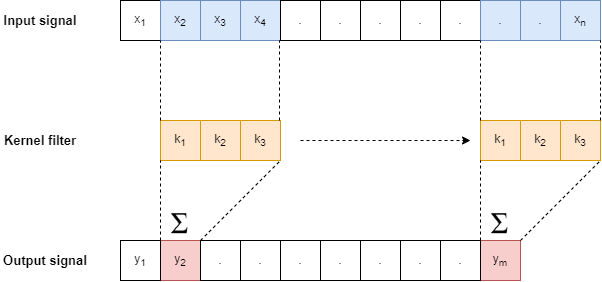
\includegraphics[width=0.6\textwidth]{Convolution.drawio.png}
  \caption{1D Convolution}
\end{figure}

\paragraph{Padding:} 
can be defined to add pixels to boundary of the signal.
In the example, padding is set to $0$ and therefore, the signal dimension is decrased by $2$.
If signal dimension should be fixed during convolution, padding is a powerful tool. For padding $1$,
the input dimension $n$ would be equal to output dimension $m$, as an extra element in the output signal
will be at boundaries.


\paragraph{Stride:}
is the parameter, how far kernel moves each time. In the example, stride was defined to be $1$.
If stride is increased, the output signal dimension will decrease.


\subsection{U-Net}
U-Net can boost performance of computed tomography reconstruction.
It is an convolutional neural network, which is well suited for image segmentation in different domains.
\cite{unet-tomography} showed great success for biomedial image segmentation.

The neural network architecture consists of contracting path and expansive path,
resulting in a U-shape, as illustrated in figure~\ref{fig:u-net-architectue}.

\begin{figure}[H]
  \centering
  \label{fig:u-net-architectue}
  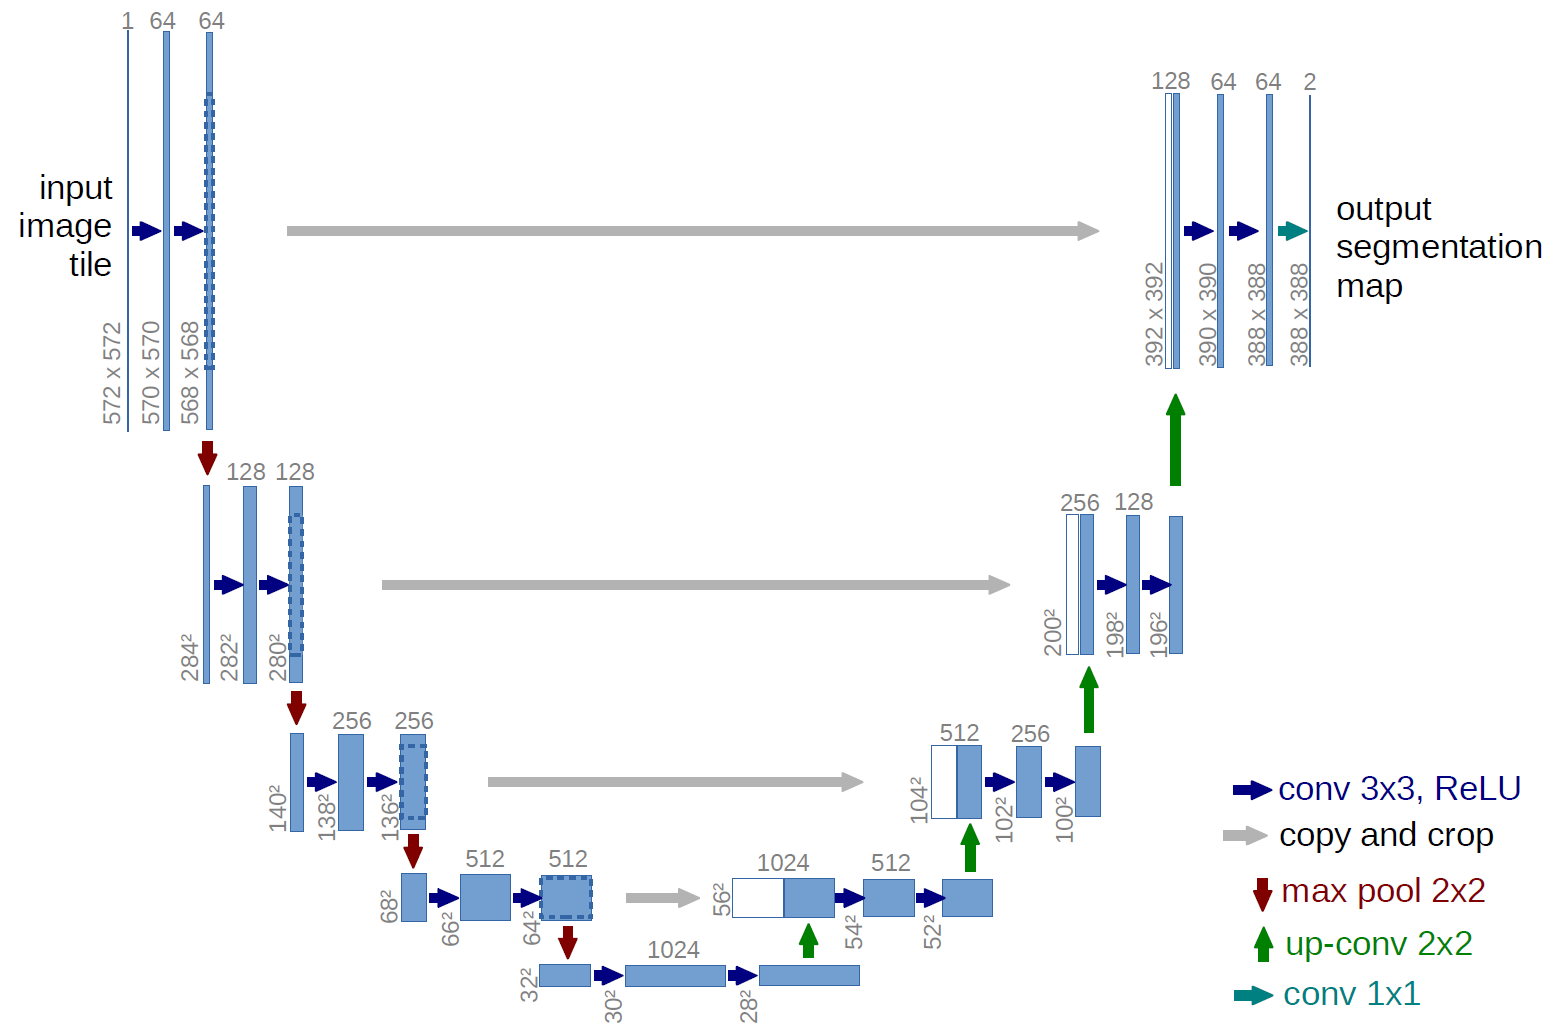
\includegraphics[width=0.6\textwidth]{u-net-architecture.png}
  \caption{
    U-Net architecture \cite[p 2, Fig. 1]{unet-tomography} \\
    Number on top of boxes denotes channels, where numbers at bottom of the box refers to input dimension.
    }
\end{figure}


In contracting path (left part), input dimension will be decreased and channels increased.
For every step in the contracting path, two 3x3 convolution layers are followed by a rectified linear unit (ReLu)
and a 2x2 max pooling for downsampling. Further, at each downsampling step, input channels are doubled.
Multiple contracting steps are combined. After last contracting step, expansive path (right part) starts
where input dimension will be increased and input channels will be decreased.
For every expansive step, an upsampling of feature map takes place, followed by a 2x2 convolution, 
which halves the number of channels. Then, concatenation with the corresponding feature
map of contracting path is done (gray arrow in figure~\ref{fig:u-net-architectue}), followed by again two 3x3 convolutions and ReLu.
Final layer is a 1x1 convolution, to map to desired output dimension and single output channel.

\section{Architecture}
\label{sec:architecture-GatDenoiser}
Now, all individual components are introduced, the GAT-Denoiser architecture can be defined.
First, the different neural network layers will be explained and second, loss and training.

As defined in equation for computed tomography \ref{eq:2Dreconstruction}, $N$ is the number of observation and
$M$ observation dimension.
Therefore, input to the network will be in $\mathbb{R}^{N \times M}$. If speaking from sinograms, 
number of observation $M$ can be seen as resolution of the sinogram. Further, $N$ is the number
of nodes of our processed, as for every observation, one node is assinged.

\subsection{Layers}

In figure~\ref{fig:architecture-detailed}, the detailed GNN architecture can be seen.
It is paremetrized with $channels$, $heads$ and $layers$. 
The number of channels in convolution can be increased with parameter $channels$.
Fruther, $heads$ determine the number of heads used in the GAT layers and parameter 
$layers$ defines how many convolution and GAT layers are stacked together.


\begin{figure}[H]
  \centering
  \label{fig:architecture-detailed}
  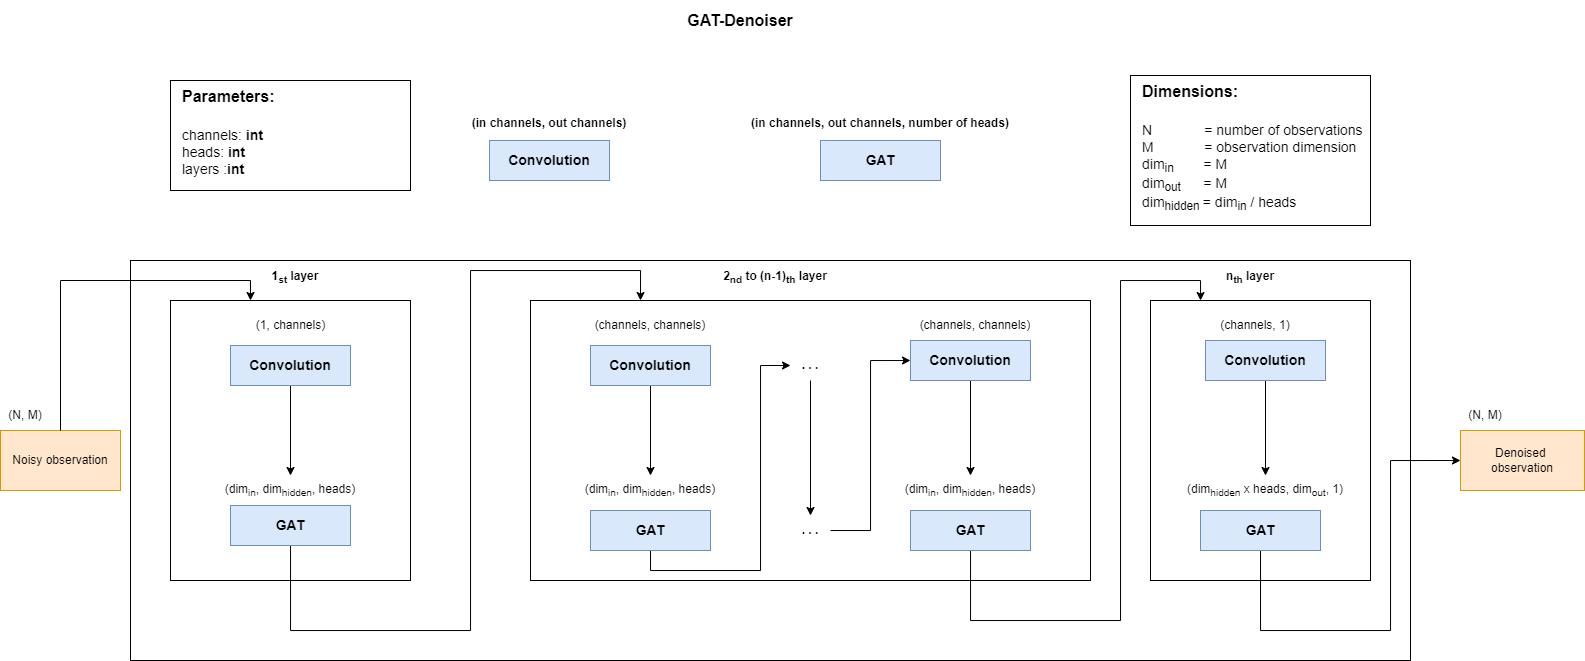
\includegraphics[width=\textwidth]{GAT_Architecture_Detail.drawio.png}
  \caption{Overall GAT-Denoiser architecture}
\end{figure}


For every layer, first convolution and then GAT is processed. 
Convolution in the whole network was defined with kernel size of 3 and padding 1,
therefore, the dimension of convolved signal will not change.
Further, additional convolutional channels can be used for learning, 
if parameter $channels > 1$, channels are increased in the first convolution layer 
and decreased in the last one.
Parameter $heads$ controls the multi-head approach for GAT. Input and hidden dimension
of GAT is $M$  if no heads are used.
If multi-head attention is used, hidden dimension will be set to $M / heads$.
In the last GAT layer, everything gets prepared for output dimension and 
averaging with 1 head is applied.




\subsection{Training}

As already mentioned, an end-to-end learning approach is used where quality of reconstruction is 
compared in the loss.

Therefore, the outcome of GAT-Denoiser is not directly part of the loss, but first reconstruction will be computed.
Reconstructions can be nicely compared with the $\ell2$-norm:

\begin{equation}
  \mathcal{L} = \parallel x_i - Recon ( \text{GAT-Denoiser}(A(x_i, \theta, s) + \eta)) \parallel ^2_2
\end{equation}

As $x_i$ is part of the loss, access to original object is needed during training.

Further, U-Net will be jointly used with FBP as reconstruction. For that to work, U-Net needs to be 
first trained with the dataset and learned model can be be pluged into GAT-Denoiser.


